Our system implements the provided spec: a pig2pig network in which pigs
collaborate to avoid impact with an adversarial bird.

\subsection{Game Map}

The game map is single-dimensional with pigs and columns placed
randomly. It is assumed that the bird is always launched from the left
(as in the original Angry Birds). The ratio of columns to pigs is at
most one.

\subsection{Assumed Physics}

We assume that certain behaviors for each element type:

\begin{itemize}
\item
  \textbf{Pig}: An impacted pig will fall to the right (as the bird
  always approaches from the left). If a pig falls onto another pig both
  are considered impacted, but the second pig does not change position
  on impact. If a pig is impacted while having a column to the right,
  then that column will also fall to the right, affecting any pig which
  may find itself in that position.
\item
  \textbf{Column}: If a column is impacted directly, then it falls to
  the right, only affecting any pig or column to its immediate right.
\end{itemize}

\subsection{Game Engine}

In our system the \emph{game engine} has several roles:

\begin{enumerate}[1.]
\item
  Map generation
\item
  Pig network topology generation
\item
  Sending round-initiating trajectory message to the nearest pig.
\item
  Ends the round.
\end{enumerate}

\subsection{Pigs as Actors}

Each pig functions as an actor which can recieve and act on several
message types, derived from the original specification:

\begin{itemize}
\item
  \texttt{Trajectory(position: Int)}
\item
  \texttt{BirdApproaching(targetPosition: Int, hopCount: Int)}
\item
  TODO: \texttt{Status(pigId: Int)}
\item
  TODO: \texttt{EndGame}
\item
  TODO: \texttt{TakeShelter(??)}
\end{itemize}

\subsection{Launching a bird}

A bird is launched is

\section{Description of ``how it works''}

\section{Design Decisions / Trade-offs}

\section{Possible Improvements}

\begin{verbatim}
[and extensions]
\end{verbatim}

\begin{itemize}
\item
  Sketch how these would be done.
\end{itemize}

\section{How to run the program}

We require \texttt{maven}, the Java dependency management tool, to pull
in all dependencies and generate a jar file of compiled code.

We have included two scripts in the code directory:

\begin{enumerate}[1.]
\item
  \textbf{\texttt{bin/install.sh}}: This will retrieve all the
  dependencies, compile the source.
\item
  \textbf{\texttt{bin/run.sh}}: This will run several rounds of the
  game, running through all of the test cases (shown on the following
  page).
\end{enumerate}

\pagebreak

\section{Test cases:}

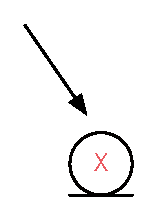
\includegraphics{figs/test1.pdf} 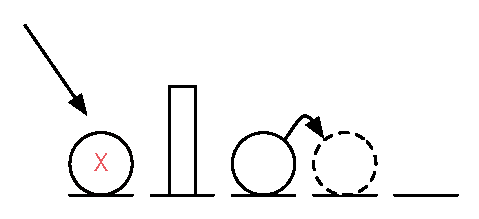
\includegraphics{figs/test2.pdf}
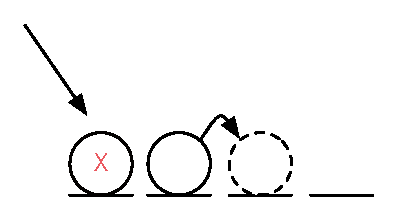
\includegraphics{figs/test3.pdf} 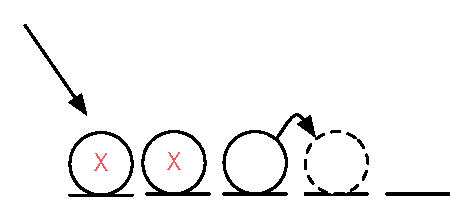
\includegraphics{figs/test4.pdf}
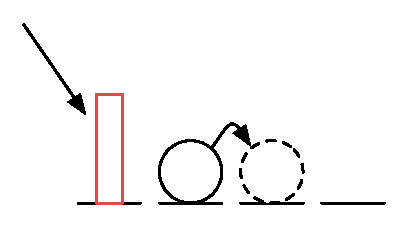
\includegraphics{figs/test5.pdf}
